\documentclass[a4paper]{article}
\usepackage[a4paper]{geometry}
\usepackage[utf8]{inputenc}
\usepackage{polski}
\usepackage[polish]{babel}
\usepackage[T1]{fontenc}
\usepackage{graphicx}
\usepackage{verbatim}
\usepackage{float}
\usepackage{minted}
\usepackage{microtype}
\usepackage{shortvrb}
\usepackage{amsmath}

\let\olditemize=\itemize \let\endolditemize=\enditemize \renewenvironment{itemize}{\olditemize \itemsep0em}{\endolditemize}

\title{TEMAT ĆWICZENIA: OpenGL – interakcja z użytkownikiem}
\author{Marcel Guzik}

\begin{document}
\section{Wprowadzenie}

Celem ćwiczenia jest ilustracja możliwości oświetlania obiektów na scenach 3D z
wykorzystaniem biblioteki OpenGL z biblioteką GLUT. W trakcie realizacji
ćwiczenia pokazano jak opisać własności materiału z którego jest wykonany
oświetlany obiekt, jak na scenie zdefiniować źródło światła i jak dobrać jego
parametry. Końcowa wersja programu realizuje sterowanie położeniem dwóch
barwnych źródeł światła oświetlających nieruchomy obiekt, wraz z możliwością
poruszania się obserwatora.


\section{Realizacja oświetlenia}

Do realizacji oświetlenia modelu wykonano dwie techniki, oświetlenie Phonga oraz
cieniowanie Phonga.

\subsection{Oświetlenie Phonga}

Oświetlenie Phonga jest modelem lokalnego oświetlenia punktów w przestrzeni
trójwymiarowej. Według tego modelu, na oświetlenie punktu składa się kombinacja
trzech różnych typów oświetlenia.

\begin{itemize}
    \item \textbf{Oświetlenie ambientowe} - Reprezentuje tzw. światło otoczenia,
          czyli światło o niskiej intensywności, które, rozproszone po całej
          scenie, pozwala na dostrzeżenie konturów obiektu. Polega na
          naniesieniu na cały obiekt jednego, dosyć ciemnego koloru.

    \item \textbf{Oświetlenie rozproszone (dyfuzyjne)} - Reprezentuje światło
          które zostało odbite od obiektu i uległo rozproszeniu. Głównie z tego
          rodzaju światła składają się obiekty matowe.

          \begin{figure}[H]
              \centering
              
\includegraphics[width=0.5\textwidth]{diffuse_light}
              \caption{Oświetlenie rozproszone. Niezależnie od kąta pod którym obserwator patrzy na powierzchnię, jest ona oświetlona równomiernie.}
          \end{figure}

    \item \textbf{Oświetlenie zwierciadlane (specular)} - Reprezentuje światło
          które uległo odbiciu zwierciadlanemu, tj. gdy kąt światła odbitego
          jest równy kątowi światła padającego. Głównie z tego rodzaju światła
          składają się obiekty błyszczące

          \begin{figure}[H]
              \centering
              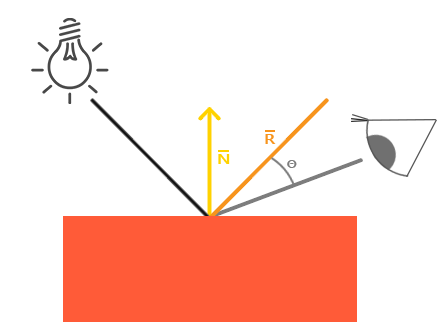
\includegraphics[width=0.5\textwidth]{specular_light}
              \caption{Oświetlenie zwierciadlane. Kąt odbicia jest równy kątowi padania. Obserwator widzi różną intensywność światła w zależności od tego jak blisko odbitego promienia się znajduje.}
          \end{figure}
\end{itemize}

\begin{figure}[H]
    \centering
    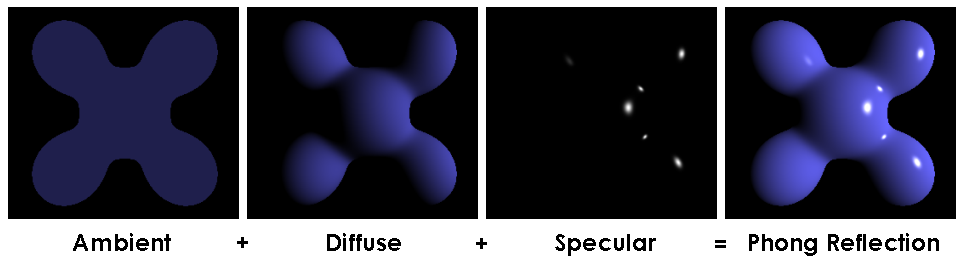
\includegraphics[width=\textwidth]{phong_reflection_model}
    \caption{Przykład zastosowania modelu oświetlenia Phonga.}
\end{figure}

\subsection{Cieniowanie Phonga}

Cieniowanie Phonga jest techniką cieniowania polegającą na interpolacji wektora
normalnego dla każdego rasteryzowanego fragmentu. Dzięki niemu uzyskujemy
``gładkie'' cieniowanie, pozbawione widocznych krawędzi i wierzchołków.

Cieniowanie Phonga bazuje na innej technice cieniowania zwanej cieniowaniem
Gourauda. W tej technice dla wierzchołków modelu obliczany jest kolor zgodnie z
modelem oświetlania Phonga, a następnie ten kolor jest interpolowany dla
fragmentów pomiędzy wierzchołkami. Wada takiego modelu pojawia się gdy odbicie
zwierciadlane pada na środek płaskiej powierzchni. Ponieważ odbicie występuje
tylko na środku powierzchni, a nie przy jej wierzchołkach, odbicie znika.
Cieniowanie Phonga eliminuje tą wadę przez to że nie interpoluje koloru, lecz
wektory normalne, a dla każdego fragmentu kolor liczony jest z osobna.


\begin{figure}[H]
    \centering
    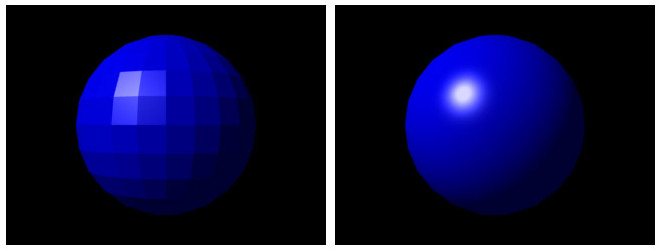
\includegraphics[width=0.8\textwidth]{phong_shading}
    \caption{Przykład cieniowania Phonga.}
\end{figure}

\section{Realizacja programu}

\subsection{Konfiguracja oświetlenia}

Oświetlenie jaja realizowane jest przez funkcje \mintinline{C}{glMaterial()} i
\mintinline{C}{glLight()}. Poniższe fragmenty znajdują się w funkcji
\verb|init()| wywoływanej raz na początku programu, i służą do konfiguracji
systemu oświetlenia.

\begin{minted}{C}
    // Ustawienie patrametrów materiału
    glMaterialfv(GL_FRONT, GL_SPECULAR, mat_specular);
    glMaterialfv(GL_FRONT, GL_AMBIENT, mat_ambient);
    glMaterialfv(GL_FRONT, GL_DIFFUSE, mat_diffuse);
    glMaterialf(GL_FRONT, GL_SHININESS, mat_shininess);
\end{minted}

Funkcje z rodziny \mintinline{C}{glMaterial()} służą do ustawiania właściwości
materiału z którego składa się obiekt. W powyższym fragmencie dla powierzchni
które widzimy z przodu (czyli w wypadku naszego jaja, z zewnątrz) ustawiamy
wartości reflektywności (czyli wartości kolorów w modelu RGBA) materiału dla
każdego z trzech typów światła w modelu oświetlenia Phonga. Ponadto parametr
\mintinline{C}{GL_SHININESS} określa jak dobrze materiał odbija światło. Im
wyższa wartość tego parametu, tym mniejszy i bardziej ``skoncentrowane'' jest
odbicie zwierciadlane.

\begin{minted}{C}
    glLightfv(GL_LIGHT0, GL_AMBIENT, light_ambient);
    glLightfv(GL_LIGHT0, GL_DIFFUSE, light_diffuse);
    glLightfv(GL_LIGHT0, GL_SPECULAR, light_specular);

    float pos[4] = {0.0, 0.0, 0.0, 1.0};
    angles_to_coords(light0Angles, pos);
    glLightfv(GL_LIGHT0, GL_POSITION, pos);

    glLightf(GL_LIGHT0, GL_CONSTANT_ATTENUATION, att_constant);
    glLightf(GL_LIGHT0, GL_LINEAR_ATTENUATION, att_linear);
    glLightf(GL_LIGHT0, GL_QUADRATIC_ATTENUATION, att_quadratic);
\end{minted}

Następnie ustawiamy wartości koloru światła oraz jego pozycję za pomocą funkcji
\mintinline{C}{glLightfv()} oraz jej parametrów \verb|GL_AMBIENT|,
\verb|GL_DIFFUSE|, \verb|GL_SPECULAR| oraz \verb|GL_POSITION|. Następnie
parametry \verb|GL_CONSTANT_ATTENUATION|, \verb|GL_LINEAR_ATTENUATION| i
\verb|GL_QUADRATIC_ATTENUATION| służą do modyfikacji intensywności światła
jeżeli jest to światło punktowe a nie kierunkowe.

Powyższy fragment odpowiada za skonfigurowanie pierwszego światła, czerwonego.
Fragment ten powtórzony jest dla drugiego światła, które świeci na kolor
niebieski.

\begin{minted}{C}
    glShadeModel(GL_SMOOTH); // właczenie łagodnego cieniowania
    glEnable(GL_LIGHTING);   // włączenie oświetlenia
    glEnable(GL_LIGHT0);     // włączenie źródła o numerze 0
    glEnable(GL_LIGHT1);     // włączenie źródła o numerze 1
\end{minted}

Na koniec wybieramy model gładkiego cieniowania oraz włączamy oświetlanie OpenGL
oraz oba nasze światła.

\subsection{Generowanie wektorów normalnych}

Aby możliwe było oświetlenie powierzchni jaja, niezbędne było wyliczenie
wektorów normalnych dla wszystkich jego wierzchołków. W tym celu przekształcono
odpowiednio równania parametryczne użyte przy obliczaniu wierzchołków.

\begin{figure}[H]
    \centering
    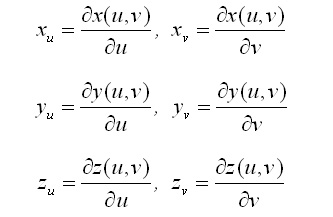
\includegraphics[width=0.5\textwidth]{wzor_4}
\end{figure}
\begin{figure}[H]
    \centering
    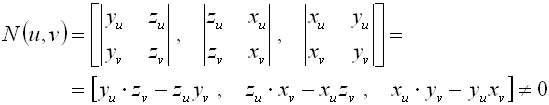
\includegraphics[width=0.8\textwidth]{wzor_3}
\end{figure}
\begin{figure}[H]
    \centering
    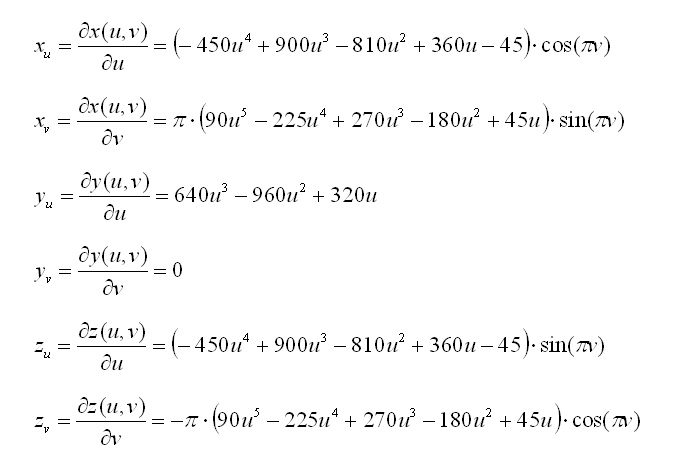
\includegraphics[width=0.8\textwidth,height=7cm]{wzor_5}
\end{figure}

\subsection{Rezultat}

\begin{figure}[H]
    \centering
    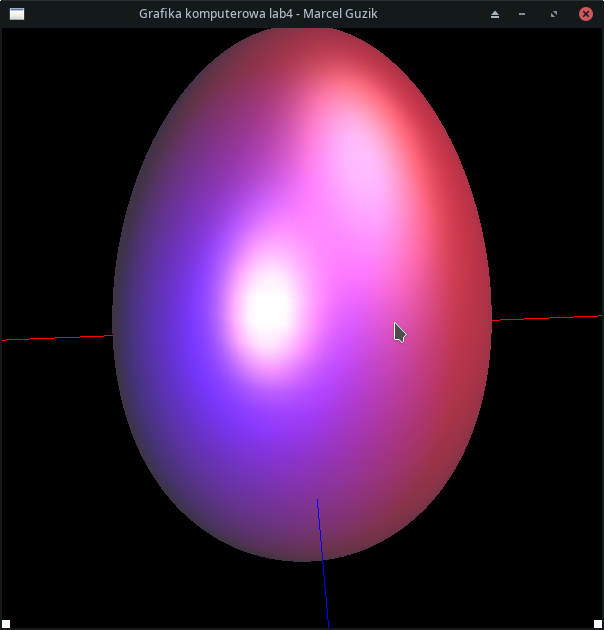
\includegraphics[width=0.6\textwidth]{result}
\end{figure}

\section{Podsumowanie}

Zadanie zaprezentowało możliwości realizacji oświetlenia i cieniowania w
bibliotece OpenGL. Możliwe jest poruszanie źródłami światła oraz obserwatorem po
powierzchni jaja, a także ich przybliżanie i oddalanie.

\end{document}